\chapter{Introduction}
\label{ch:intro}
\tab{\Large This section gives a scope description and overview of everything included in this SRS document. Also the purpose of this document is described and a list of abbreviations and definitions is provided.}
\section{Purpose}
\tab{The purpose of this document is to give a detailed description of the requirements of the "“RAMPAGE“" software (game).It will illustrate the purpose and complete declaration for the development of system. It will also explain constraints, interface and interactions with users and external applications. This document is primary intended to be proposed to a customer for its approval and a reference for describing the first version of the system for the development team.}
\section{Document Conventions}
%\begin{table}
	%\resziebox{\textwidth}{!}{%
	\begin{tabu} to 1.0\textwidth{|X[l]|X[r]|}
		\hline
		Term & Definitions\\
		\hline\hline
		Users/players & Someone who interacts with the system\\
		\hline
		Fps & First Person Shooter\\
		\hline
	\end{tabu}
%\end{table}
%\section{Intended Audience and Reading Suggestions}
\section{Product Scope}
\tab{"RAMPAGE"” is a multiplayer, fps, horror game mainly designed for people with greater than 16 years .It is for entertainment purpose only. Players can join by lobby and play game.}
\section{References}
{\begin{enumerate}
	\item https://unity3d.com/learn/tutorials
	\item https://www.assetstore.unity3d.com/en/\#
	\item https://en.wikipedia.org/wiki/Perlin\_noise
\end{enumerate}}

\chapter{Overall Description}
\label{Overall Description}
\tab{\Large This section will give an overview of the whole system. The system will be explained in its context to show how the system interacts with another system and introduce the basic functionality of it. It will also describe what type of stakeholders that will use the system and what functionality is available for each type. At last, the constraints and assumptions for the system will be presented. }

\section{Product Perspective}
\tab{"RAMPAGE"" is mostly aimed at users aged between 16 and 60. It is simply a shoot-to-survive game, with realistic graphcis and dark music and environment to appease those looking for some action in the screen.}

\section{Product Functions}
\tab{The key features in the game are:
 \begin{itemize}
 	\item Menu driven GUI Interface
 	\item Enemies having AI
 	\item Lobby creation for multiplayer
 	\item Dark graphis and music for environment
 \end{itemize}

\section{User Classes and Characteristics}
\tab{There are only one type of users in this system, the players. Players interact with the system with the help of GUI interface.}

\section{Operating Environment}
\tab{This game is targeted for the Windows environment, preferably Windows 7 and above. DirectX10 and above is mandatory too.}

\section{Design and Implementation Constraints}
\tab{The network connection is a constraint for the application. Since the application fetches data from the database over the internet. It is crucial that there is an Internet connection for the application to function.}\\
\tab {Power failure is also a constraint, as there is a multiplayer game, so there is no saving option.}

\section{User Documentation}
\tab{This product is under development state and requires a complete implemented prototype to explain the user documentation.}

\section{Assumptions and Dependencies}
\tab{Our assumption about the product is that it will always be used on Windows OS and pc having enough capability to run this application smoothly.}\\
\tab{Another assumption is that there is always a good Internet connection.}

\newpage




\chapter{Specific Requirements}
\label{Specific Requirements}
\tab{\Large This section contains all of the functional and quality requirements of the system. It gives a detailed description of the system and all its features.}
\section{External Interface Requirements}
\tab{This section provides a detailed description of all inputs into and outputs from the system. It also gives a description of the hardware, software and communication interfaces and provides basic prototypes of the user interface.}
\subsection{User Interfaces}
\tab{Some of the intended looks for the GUI of the game is as given below:}
\begin{figure}[H]
\centering
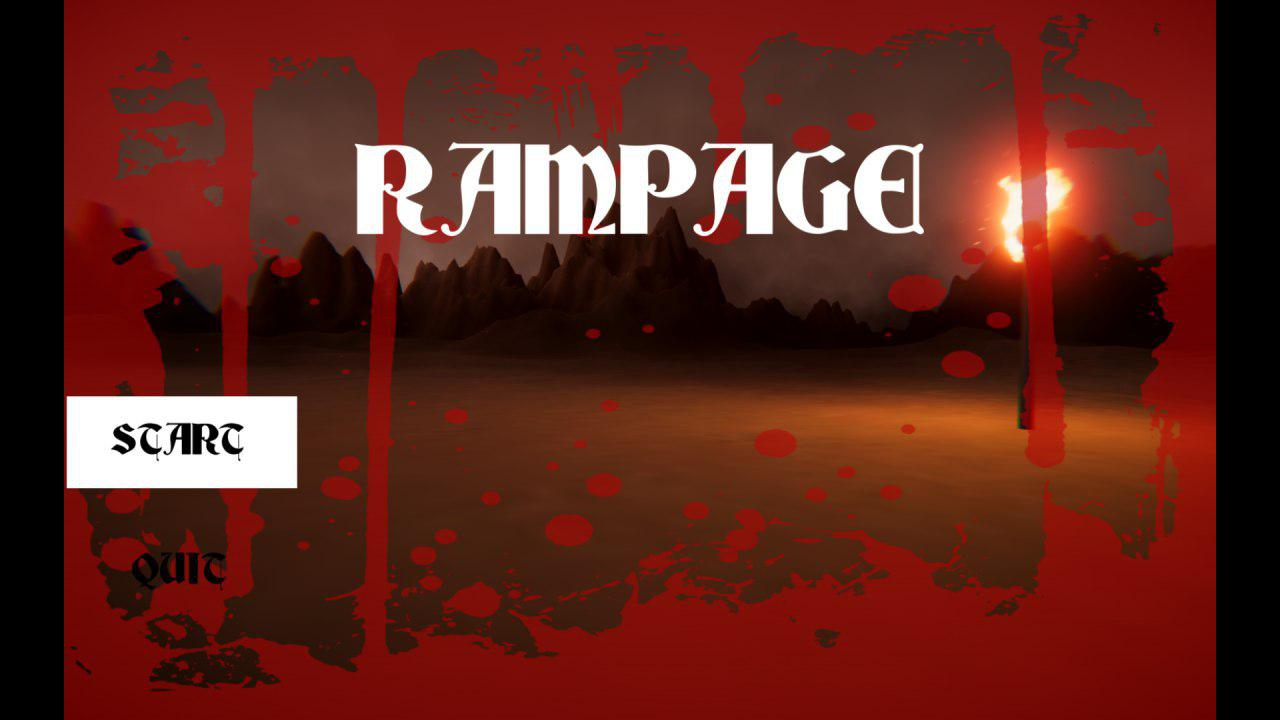
\includegraphics[width=460pt,height=\textheight,keepaspectratio]{./images/1.jpg}

\end{figure}
\subsection{Hardware Interfaces}
\tab{No specific hardware components required. However, the ones mentioned below are mandatory:
	\begin{itemize}
		\item Basic PC setup
		\item Good Headphones
	\end{itemize}
\subsection{Software Interfaces}
\tab{It uses mostly C\# language for coding, Unity game engine for developing the game and Blender for graphical models.}
%\section{Communications Interfaces}


%\chapter{System Features}
%\label{System Features}

%\section{System Feature 1}
\section{Functional Requirements}
\tab{The functional requirements of the game are as follows:
 \begin{itemize}
 \item Dark Environment: Being a horror game, this is a must. It can be achieved by using a dark landscape and lack of lighting.
 \item Game Menu for User Interaction: Like most games, a proper menu for navigation around the game is a necessity.
 \item Shooting: Player must be able to shoot at enemies and survive waves of death.
 \item Realistic graphics and gameplay: Unity engine and Blender make this look easy, with best quality shaders and rendering.
 \item Tough enemies: The toughness of the enemies is to be set up in the code.
 \item Artificial Intelligence for the Enemies: To avoid making it look too easy, some intelligence is to be planted in the enemies.
 \item User health: On taking hits from the enemies, the user will be taking damage, and hence a health bar is placed to notify the player of their current health.
 \item Terrain Generation: The terrain shall be dynamically generated, and only the immediate terrain in the vicinity of the player shall be visible, hence loading time shall be less and the application won't be heavy on the resources.
 \end{itemize}
\section{Other Nonfunctional Requirements}
%\label{Other Nonfunctional Requirements}

\subsection{Performance Requirements}
\tab{The game will run without any lag on a PC running Windows 7 and above, with at least 4 GB RAM, and a 2 GB AMD Radeon or similar graphics card. For best performance, use an 8 GB RAM with 4 GB Nvidia G-series, with a resolution of 1366 x 768.}
\subsection{Safety Requirements}
\tab{Since there are lots of flashy objects and movements, some users might face headaches, nausea or similar symptoms. If you are epileptic, please stop the game and get medical help.}
\subsection{Security Requirements}
\tab{There are no possible ways to hack or break the game. User information is not recorded at any point.}
%\section{Software Quality Attributes}
%\section{Business Rules}

\section{Other Requirements}
%\label{Other Requirements}
\subsection{Legal Requirements}

\begin{appendices}
\chapter{Glossary}
\chapter{Analysis Models}
\chapter{To Be Determined List}


\end{appendices}


